\documentclass{edm_template}

\begin{document}

\title{Choosing Training Data Size for Bayesian Knowledge Tracing Models
\titlenote{Class report for INFO 290: Educational Data Mining (Spring 2014), led by Zachary A. Pardos at University of California, Berkeley. This is not a peer-reviewed work.}}
%\subtitle{[Extended Abstract]
%\titlenote{A full version of this paper is available as
%\textit{Author's Guide to Preparing ACM SIG Proceedings Using
%\LaTeX$2_\epsilon$\ and BibTeX} at
%\texttt{www.acm.org/eaddress.htm}}}

\numberofauthors{1}
\author{
\alignauthor
Derrick Coetzee\\
       \affaddr{University of California, Berkeley}\\
       \email{dcoetzee@berkeley.edu}
}

\maketitle
\begin{abstract}
An important question in the practical application of Bayesian knowledge
tracing models is determining how much data is needed to infer
parameters accurately. If training data is inadequate, even a perfect
inference algorithm will produce parameters with poor predictive
power. In this work, we describe an empirical study using synthetic
data that provides estimates of the accuracy of inferred parameters
based on factors such as the number of students used to train the model,
and the values of the underlying generating parameters. We find that
the standard deviation of the error is proportional to $1/\sqrt{n}$ where
$n$ is the sample size, and that model parameters near 0 and 1 are easier
to learn accurately.
\end{abstract}

%% A category with the (minimum) three required fields
%\category{H.4}{Information Systems Applications}{Miscellaneous}
%%A category including the fourth, optional field follows...
%\category{D.2.8}{Software Engineering}{Metrics}[complexity measures, performance measures]
%
%\terms{Theory}

\keywords{BKT,knowledge tracing,sample size,empirical}

\section{Introduction}
Simple Bayesian knowledge tracing models a student's observed responses to a sequence of items
as a Markov process, with their knowledge state as a hidden underlying variable. If values
are given for the four standard parameters, learning rate, prior, guess, and slip, the
likelihood of a particular set of response sequences can be computed. Using standard search
procedures like expectation maximization (EM), the parameter set giving the highest likelihood
for a given set of sequences can be determined, provided that the procedure converges to the global
maximum.

However, even if the procedure identifies the global maximum correctly and precisely, the resulting
parameters may not reflect the actual parameters that generated the data; this is a \emph{sampling error}
effect. It's clearest with very small samples, such as samples of size 1, but exists with larger samples as well. Empirical studies with synthetic data generated from known parameters show that the inferred parameters for a given data set can differ substantially from the generating parameters, and this same issue would arise in real settings. An understanding of the magnitude of sampling error in a particular scenario
can help to explain why the resulting model does or does make effective predictions. Moreover, if the
distribution of possible generating parameter values is known, a corresponding distribution of possible prediction values can be produced, allowing uncertainty of predictions to be expressed.

\section{Related work}
For simple problems, such as identifying mean value of a parameter in a population, or the proportion of the population falling into a subgroup, there are simple and well-understood statistical approaches for determining sample size and computing confidence intervals based on statistical power. Such approaches are not immediately applicable to the problem of minimizing the HMM error function because of its complexity and high dimensionality.

We were not able to identify any prior research into the relationship between training data size and accuracy of inferred parameters in BKT, but studies have noted that training time increases linearly with the size of the training set~\cite{falakmasir2013spectral}. Choosing an appropriate sample size for a certain desired level of accuracy can thus help to reduce training time, which is important in some real-time interactive tutor applications.

% A number of prior works using knowledge tracing models trained with relatively small numbers of students, such as 222~\cite{falakmasir2013spectral}, which our work suggests is not enough to achieve reasonable accuracy in any parameter.

De Sande~\cite{vandesande2013} has suggested that as samples become larger, models with small parameter sets  may no longer be rich enough to capture their complexity. Thus our exclusive reliance on a simple four-parameter BKT model is a limitation of our approach.

\section{Results}

In our experiments we relied on a simple standard knowledge tracing model with four parameters: learning rate, prior, guess and slip. There is only one value for each parameter, and no specialization by student or problem. Each synthetic student responded to five items; we do not vary this parameter in this study, although
intuitively having more problems per student should increase accuracy.

\subsection{Variance by parameters in one-parameter system}
\label{variance1}

First, for each of the four parameters, we hold the other parameters at zero (except for learning rate, which we hold at 0.5 to avoid a trivial system) and vary the remaining parameter. We hold the number of students fixed at 1000, which is large enough to consistently produce a standard deviation not exceeding 2\% (this is necessary to avoid the boundary effects which accompany very large variances).

Next, for each value of the varying parameter, we use the corresponding model to generate 1000 random samples of 1000 students each, and for each one we use EM to find the parameter set giving the maximum log-likelihood value. EM is run starting at the generating parameters and run until fully converged (within $10^{-12}$). Starting at the generating parameters is not feasible in a realistic setting, but here it allows EM to run quickly and consistently reach the global minimum.

The mean of these inferred parameter sets was found to be close to the generating parameters (consistently $< 0.001$ absolute difference). For each parameter and each value of the parameter, the standard deviation of the 1000 parameter values inferred from the 1000 samples was measured, and is shown in Figure~\ref{fig:variance1}. These variances remained stable under repeated runs.

\begin{figure}
\label{fig:variance1}
\centering
%\includegraphics[width=1.0\textwidth]{col1.pdf}
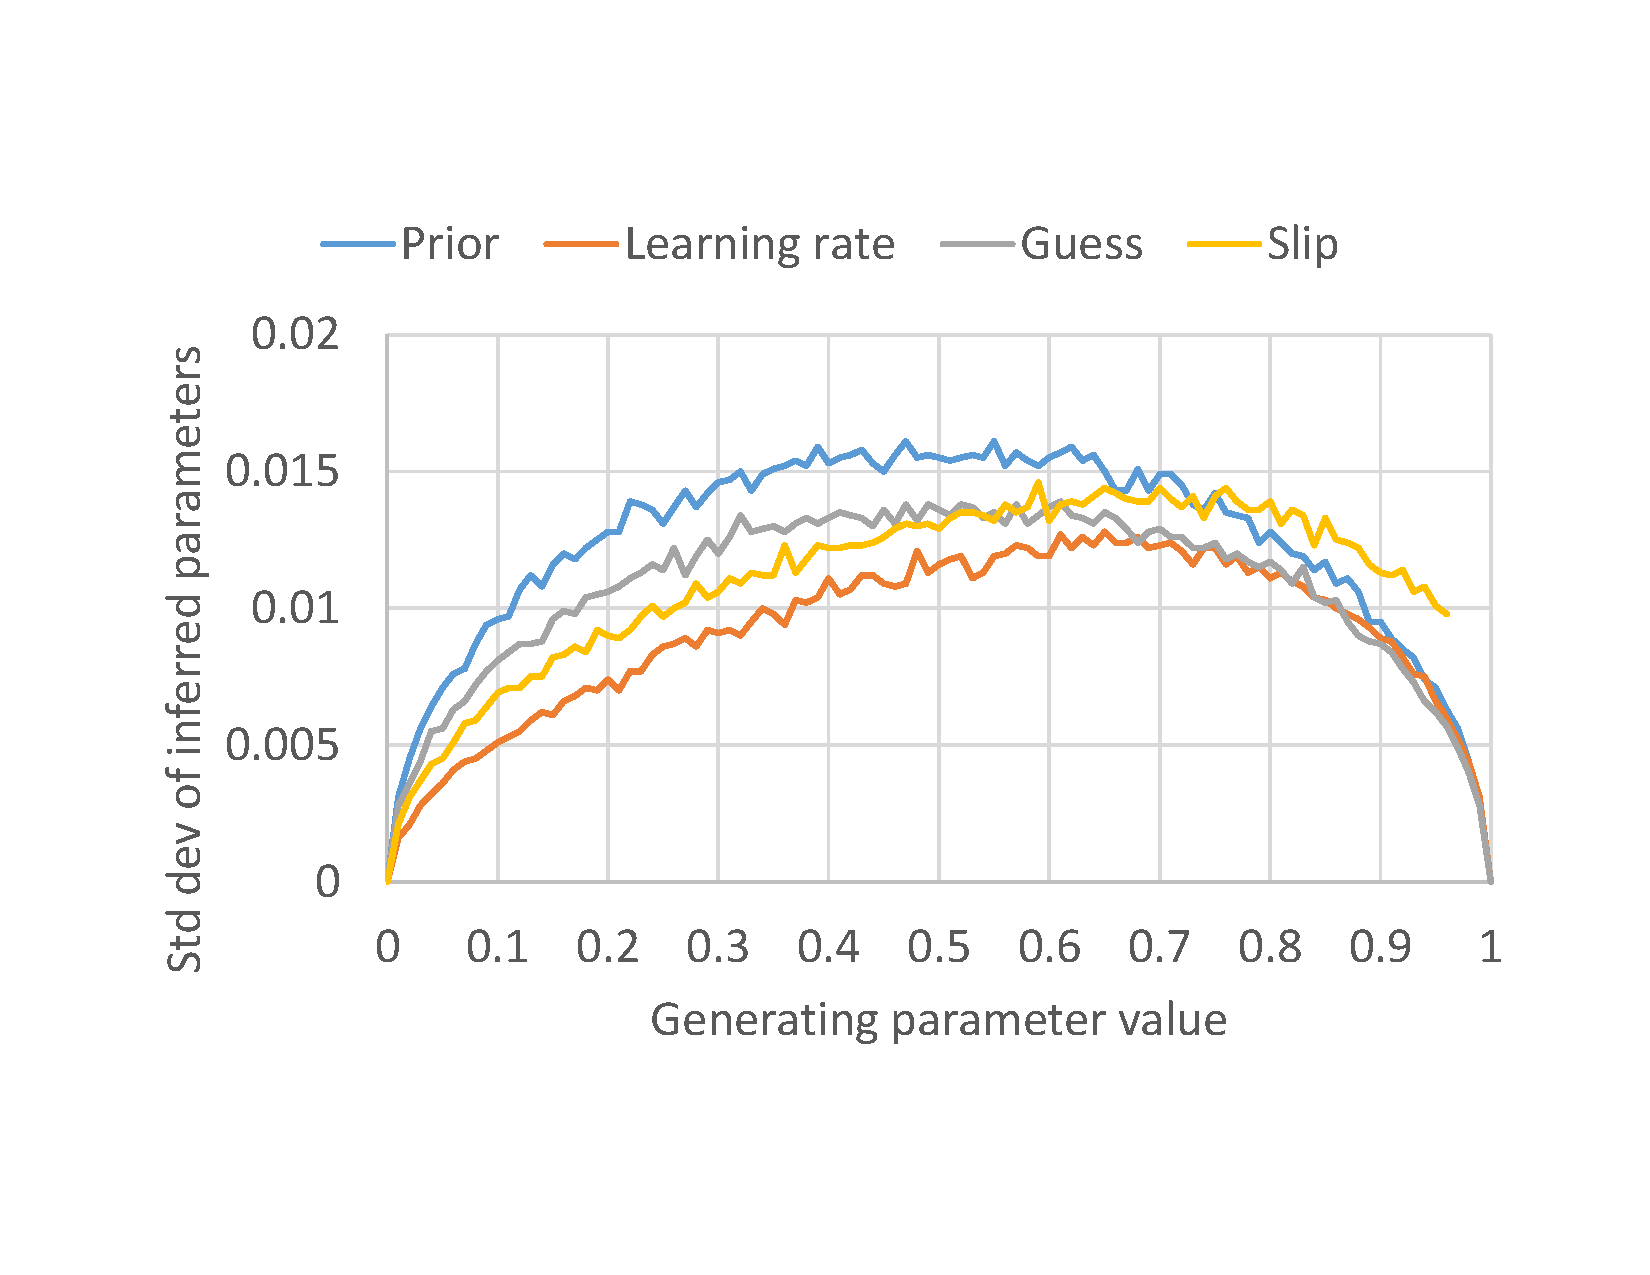
\includegraphics[width=0.5\textwidth]{data/variance1.pdf}
\caption{Accuracy of inferred parameters, based on underlying generating parameter. For values close to 0 or 1, accuracy tends to be good, while for values near 0.5 it's poor. Each parameter exhibits a different relationship, with prior exhibiting the worst accuracy, and learning rate having an asymmetric curve that's worst around 0.67. Slip is unique in having poor accuracy near 1.}
\end{figure}

\subsection{Interactions between parameters}
\label{variance2}

The accuracy of an inferred parameter depends not only on the value of that parameter, but also the values of other parameters. As a compelling demonstration of this, we examine the case where learning rate is fixed at 0.5 and slip is varied from 0 to 1, but instead of examining the accuracy of slip, we examine the accuracy of learning rate. The error in learning rate increases sharply as slip increases, as shown in Figure~\ref{fig:variance2}. This is also a possible explanation for the effect in Figure~\ref{fig:variance1} in which slip error does not converge to zero as slip approaches 1; the large error in the learning rate may prevent it from being inferred correctly.

\begin{figure}
\label{fig:variance2}
\centering
%\includegraphics[width=1.0\textwidth]{col1.pdf}
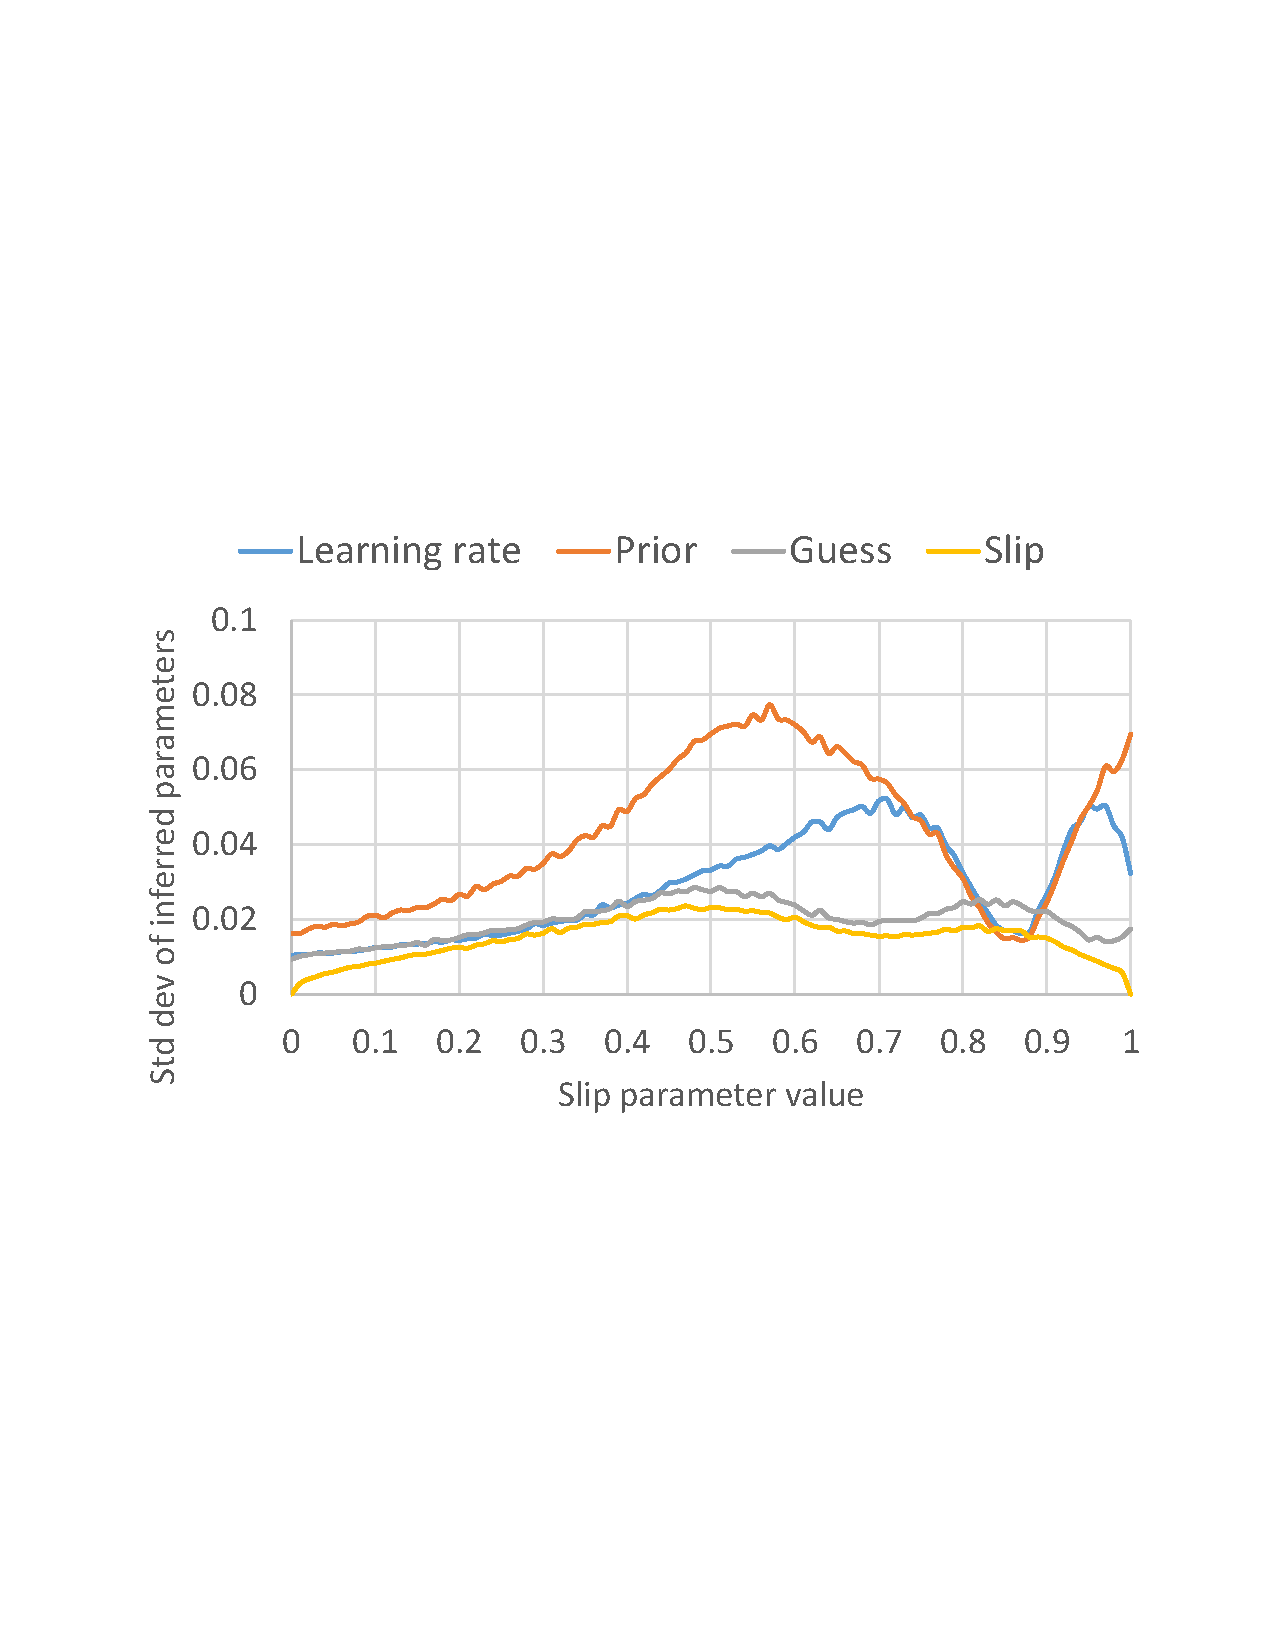
\includegraphics[width=0.5\textwidth]{data/variance2.pdf}
\caption{Error in the learning rate parameter increases sharply as the slip parameter increases, especially as it approaches 1, indicating an interaction between parameters - by the time slip reaches 0.9, the 95\% confidence interval for learning rate is already 40 percentage points wide.}
\end{figure}

\subsection{Variance by number of students with fixed parameters}

We fix the parameters at the values empirically determined in section~\ref{variance1} to give maximum variance (roughly based on the maximums of the curves, with prior and guess at 0.5, and learning rate and slip at 0.67). Because section~\ref{variance2} suggests that there are interactions between some parameters, this may not give the worst-case variance possible of all combinations, but it is a reasonable starting point for realistic values.

Next, we vary the sample size in powers of two from 2 to . For each, we perform 1000 samples of that size, verify that the mean error is near zero, and measure and plot the standard deviation of the error in all four parameters. Figure~\ref{fig:variance3} shows the result, suggesting that the standard deviation of the error is proportional to $1/\sqrt{n}$.

\begin{figure}
\label{fig:variance3}
\centering
%\includegraphics[width=1.0\textwidth]{col1.pdf}
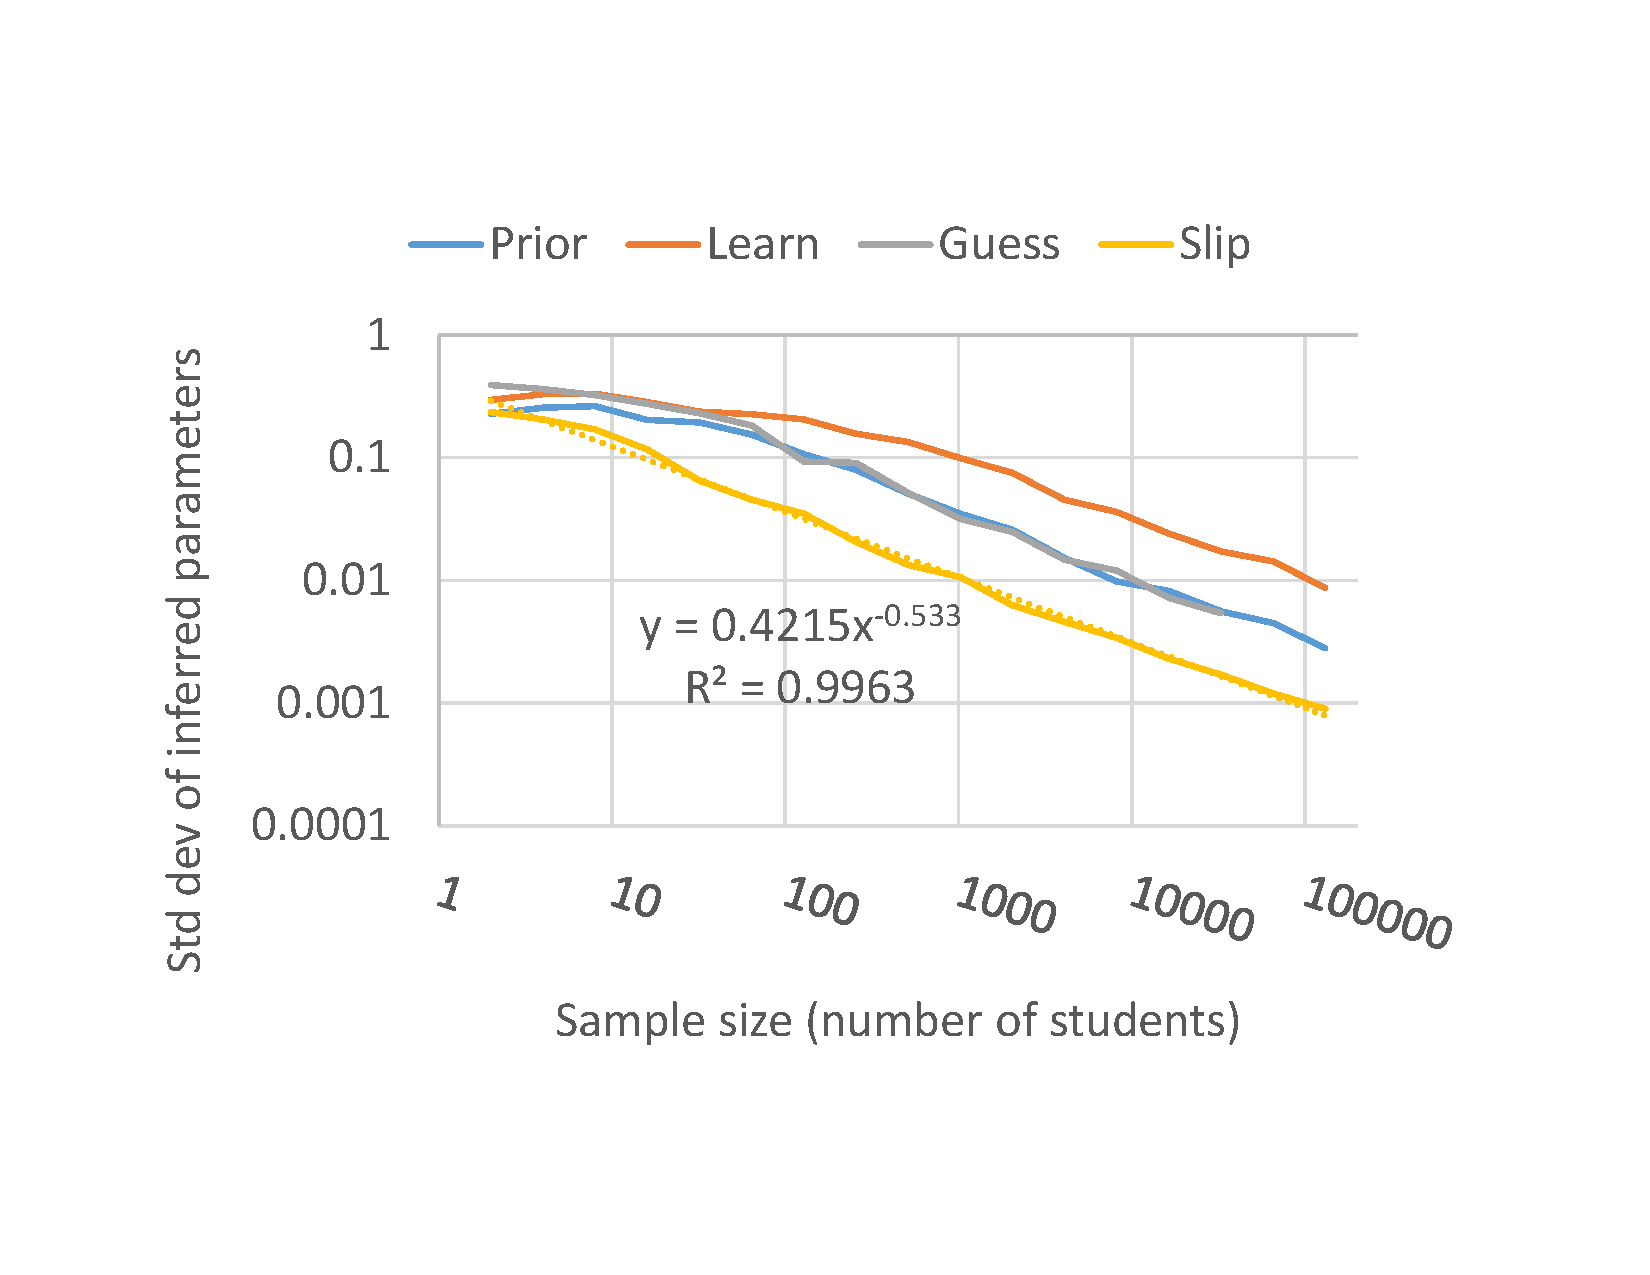
\includegraphics[width=0.5\textwidth]{data/variance3.pdf}
\caption{Accuracy of inferred parameters, based on sample size (training set size), with fixed parameters (prior=guess=0.5, learning=slip=0.67). Note that this is a log-log plot, and the lines each have slope of roughly -0.5, indicating that the standard deviation of the error is proportional to $1/\sqrt{n}$, where
$n$ is the sample size. Slip is consistently inferred most accurately, learning rate is inferred least accurately, and guess and prior are between the two and are similar.}
\end{figure}

\section{Discussion}

The results in Figure~\label{fig:variance1} can be interpreted intuitively in terms of how much information a given data set provides about each of the parameters. The model uses the learning rate, guess, and slip parameters for every problem, but only uses the prior once at the beginning; so it's not surprising that the prior is the hardest parameter to learn accurately. Because our single-parameter models for guess and slip had prior set to zero and learning rate to 0.5, knowledge had to first be learned (and relatively slowly) before there was an opportunity for slipping; hence there's more information available about the guess rate than the slip rate.

Because accuracy is good for parameter values near 0 and 1, this implies that for large enough samples, boundary effects (in which the distribution of error is skewed because values outside of the 0-1 range are not permitted) are not a serious concern. Intuitively, this behavior is expected because extremal values
tend to generate a unique signature that is recognizable and can be attributed to a single parameter.
For example, guess values near 1 lead to many observations of correct responses before sufficient opportunities for learning have occurred.

The interaction between learning rate and slip in particular can be understood because when guess is zero and slip is very high, learning is very difficult to detect (almost all responses will be incorrect regardless of whether they have learned it or not). This is just one example, and other more subtle interactions could remain yet unknown.

The main result that standard deviation is proportional to $1/\sqrt{n}$ suggests that, in order to decrease confidence interval size by a factor of 2, an increase in sample size by a factor of 4 is required. Additionally, Figure~\ref{fig:variance3} shows that acceptable error in the learning rate (at least one valid significant digit) is only achieved for sample sizes of 1000 students or more. This suggests that studies using BKT with less than 1000 students should be considered carefully for sampling error.

\subsection{Generating confidence intervals}

Provided that the sample size is large enough, the distribution can be approximated well by a normal
distribution, and the standard deviations computed in synthetic simulations such as the preceding ones
can be used to compute confidence intervals in the usual manner containing the true generating parameters (e.g. 95\% of possible values are within two standard deviations). Parameters used in these simulations can be set either by using domain knowledge, and/or by conservatively selecting values that give worst accuracy, as we did.

\section{Conclusions and Future Work}

We've only explored a small part of the space of input parameters that can affect inferred parameter accuracy; the possible interactions between parameters are not fully understood. It would also be useful
to examine different sizes of problem sets, scenarios where different students complete different numbers
of problems, models where parameters such as learning rate and guess/slip are per problem, and models where priors are measured per student (as in Pardos and Heffernan~\cite{conf/um/PardosH10}).

Although it seems intuitive that insufficient sample size can lead to poor parameter estimates with poor predictive power, this deserves verification: it's not clear which errors will damage prediction and which are benign. An empirical synthetic study that examines prediction accuracy could assess this cheaply. Going a step further, it would be useful to simulate an interactive tutoring system and assess a cost function that penalizes the system for both incorrect assessment of mastery, and for failing to assess mastery when it is reached. By applying weights to these error types, the simulation could simulate the real-world cost of inaccurate parameters in such a system.

Another important direction is extending our results to real-world data. There are a few approaches to this. One is to use a very large data set and use its inferred parameters as the ground-truth generating parameters, then examine smaller subsets to determine whether parameters are inferred less accurately. If the BKT model is appropriate, we expect to observe similar relationships between sample size and variance as with our synthetic data. Another approach would be a survey of BKT applications, to identify whether there is a consistent relationship between sample size and reported prediction accuracy. A final approach would be a controlled experiment in which two groups of very different sizes each use an ITS, the BKT is trained on the resulting data, and then the groups continue to use the ITS and their learning performance is examined (note however that asymmetric group sizes limit statistical power).

Finally, an analytical model that can explain our empirical results---such as the distinctive smooth curves observed in the variances for our simple one-parameter models---would be a valuable contribution.

%ACKNOWLEDGMENTS are optional
%\section{Acknowledgments}
%This section is optional; it is a location for you
%to acknowledge grants, funding, editing assistance and
%what have you.  In the present case, for example, the
%authors would like to thank Gerald Murray of ACM for
%his help in codifying this \textit{Author's Guide}
%and the \textbf{.cls} and \textbf{.tex} files that it describes.

\bibliographystyle{abbrv}
\bibliography{hw2ext}
\end{document}
